%
% section 6.2.2
%
\subsection{Υπηρεσία Μεταφοράς Αρχείων (FTP, TFTP)}

Και τα δύο αυτά πρωτόκολλα ασχολούνται με τη μεταφορά αρχείων μεταξύ δύο συστημάτων που συνδέονται σε ένα δίκτυο τεχνολογίας TCP/IP.

Το \emph{FTP, File Transfer Protocol} ή Πρωτόκολλο Μεταφοράς Αρχείων χρησιμοποιείται για αποστολή / λήψη αρχείων από ένα απομακρυσμένο εξυπηρετητή. Το FTP πραγματοποιεί δυο συνδέσεις μεταξύ του πελάτη και του εξυπηρετητή: στη μια μεταφέρονται εντολές και πληροφορίες ελέγχου και στην άλλη τα δεδομένα που πρόκειται να μεταφερθούν. Για να γίνει ταυτοποίηση του χρήστη που συνδέεται, γίνεται χρήση ονόματος (username) και κωδικού πρόσβασης (password). Με την ολοκλήρωση της διαδικασίας εισόδου, ο χρήστης μπορεί να επιλέξει και να μεταφέρει τα αρχεία που επιθυμεί. Το FTP μπορεί να χειριστεί τόσο αρχεία απλού κειμένου (text) όσο και δυαδικά (binary). Οι εντολές και τα δεδομένα ελέγχου μεταφέρονται μέσα από τη θύρα 21 που ενεργοποιείται κατά την έναρξη της σύνδεσης. Τα δεδομένα μεταφέρονται από τη θύρα 20.

\begin{figure}[!ht]
 \centering
 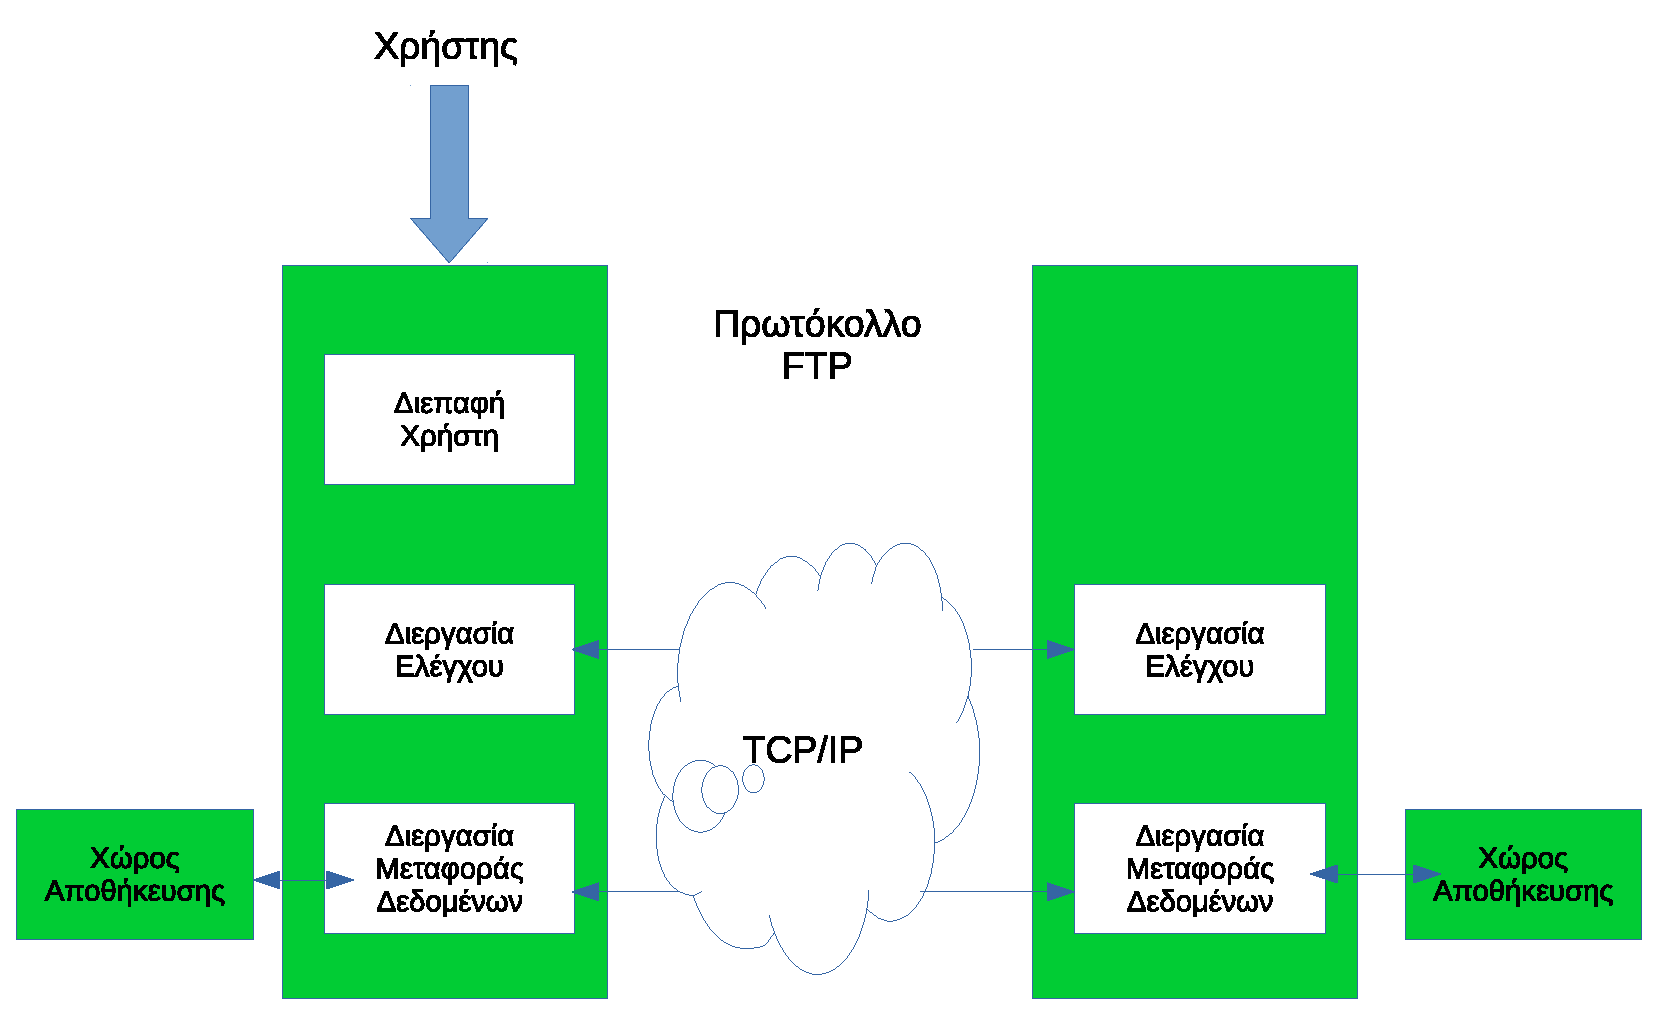
\includegraphics[width=0.85\textwidth]{images/chapter6/6-8}
 \caption {\textsl{Μοντέλο Λειτουργίας FTP}}
 \label{6-8}
\end{figure}

\begin{inthebox}
\textbf{Τι μειονέκτημα έχει το FTP στις μέρες μας;}

To FTP (όπως και το mail) είναι  από τα πλέον παλιά πρωτόκολλα εφαρμογής της τεχνολογίας TCP/IP. Την εποχή που φτιάχτηκε ο κόσμος ήταν αρκετά πιο ``αθώος'' από σήμερα. Το FTP μεταφέρει όλες τις πληροφορίες του χωρίς κανένα είδος κρυπτογράφησης. Ακόμα και το όνομα χρήστη και ο κωδικός πρόσβασης μεταφέρονται σαν απλό κείμενο μέσα από τις γραμμές του δικτύου. Αυτό φυσικά σημαίνει ότι στις μέρες μας οποιοσδήποτε θα μπορούσε να τα υποκλέψει. Για το λόγο αυτό σήμερα το FTP σπάνια χρησιμοποιείται με πραγματικούς κωδικούς πρόσβασης (έχει αντικατασταθεί για το σκοπό αυτό με άλλες ασφαλείς παραλλαγές). Σήμερα χρησιμοποιούμε περισσότερο το \emph{ανώνυμο} FTP όπου συνδεόμαστε σε ένα εξυπηρετητή ουσιαστικά χωρίς να έχουμε λογαριασμό (ως επισκέπτες) αλλά και χωρίς να έχουμε δικαιώματα πέρα από το να κατεβάσουμε συγκεκριμένα αρχεία που έχει επιλέξει ο διαχειριστής. Αυτού του είδους ο εξυπηρετητής συχνά είναι ρυθμισμένος να επιτρέπει πρόσβαση μόνο σε επισκέπτες και όχι σε αναγνωρισμένους χρήστες. 

\textbf{Με τι μοιάζουν οι εντολές του FTP;}

Όπως φαντάζεστε, σπάνια χρησιμοποιούμε απευθείας τις εντολές για να συνδεθούμε σε ένα εξυπηρετητή FTP. Συνήθως χρησιμοποιούμε κάποιο πρόγραμμα πελάτη όπως το filezilla (σχήμα \ref{6-9}). Ωστόσο και οι εντολές του FTP είναι απλές, όπως είδαμε και στο SMTP. Βασικές εντολές είναι η \textbf{get} για να πάρουμε ένα αρχείο, η \textbf{put} για να στείλουμε αρχείο (αν έχουμε συνδεθεί με όνομα και κωδικό) και η \textbf{cd} για να μετακινηθούμε σε άλλο κατάλογο (φάκελο). Για να δούμε τα περιεχόμενα ενός καταλόγου χρησιμοποιούμε την \textbf{ls}. Όπως φαντάζεστε, ένα γραφικό πρόγραμμα -- πελάτης απλά αναλαμβάνει να στείλει τις ίδιες αυτές εντολές για μας.\\
\end{inthebox}

\begin{figure}[!ht]
 \centering
 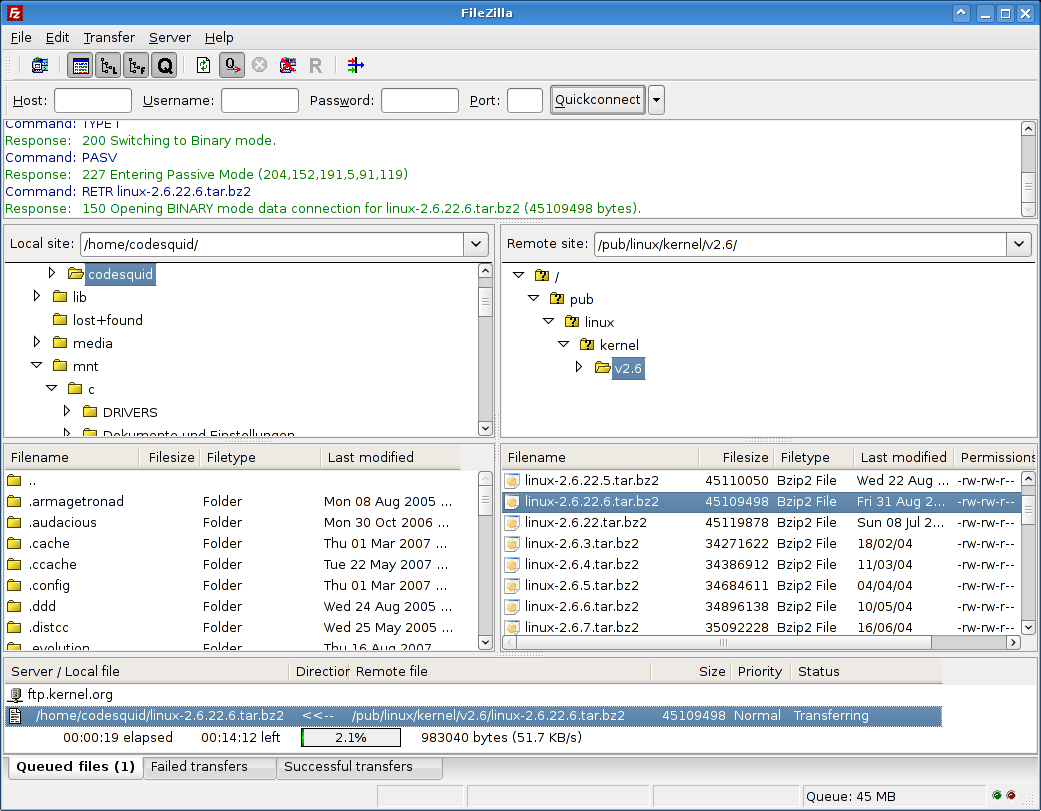
\includegraphics[width=0.85\textwidth]{images/chapter6/6-9}
 \caption {\textsl{Πρόγραμμα Πελάτης FTP (Filezilla)}}
 \label{6-9}
\end{figure}

Το πρωτόκολλο \textbf{TFTP, Trivial File Transfer Protocol} είναι μια πιο απλή εκδοχή του FTP. Μπορεί να μεταφέρει αρχεία μεταξύ πελάτη και εξυπηρετητή, αλλά δεν παρέχει έλεγχο ταυτότητας χρήστη και άλλες χρήσιμες λειτουργίες που διαθέτει το κανονικό FTP. To TFTP χρησιμοποιεί UDP στο επίπεδο μεταφοράς, ενώ το FTP χρησιμοποιεί TCP. O παρακάτω πίνακας δείχνει τις διαφορές μεταξύ των δύο πρωτοκόλλων.

\begin{tabular}{|c|c|}
\hline
\textbf{FTP (File Transfer Protocol)} & \textbf{TFTP (Trivial File Transfer Protocol)} \\
\hline
Χρησιμοποιεί το TCP & Χρησιμοποιεί το UDP    \\
στο επίπεδο μεταφοράς & στο επίπεδο μεταφοράς \\
\hline
Χρησιμοποιεί ισχυρές & Χρησιμοποιεί απλές \\
 εντολές ελέγχου &  εντολές ελέγχου \\
\hline
Στέλνει δεδομένα και εντολές & Δεν χρησιμοποιεί συνδέσεις \\
από χωριστές συνδέσεις TCP   & γιατί το UDP είναι πρωτόκολλο \\
& χωρίς σύνδεση \\
\hline
Απαιτεί περισσότερη μνήμη & Απαιτεί λιγότερη μνήμη \\ 
και υπολογιστική ισχύ &  και υπολογιστική ισχύ \\
\hline
\end{tabular}